In order to simulate quantum systems at finite temperatures, we need to construct statistical ensembles from the quantum states. An useful quantity is the density matrix $\rho$.


\begin{equation}
    \begin{split}
        Z &= e^{ - \beta E_n} \\
          &= \sum_n \Braket{n | e^{ - \beta \hat{H} }  | n} \\
          &= \Tr( e^{ - \beta \hat{H} } )
    \end{split}
\end{equation}

\begin{equation}
    \begin{split}
        \rho &= \sum_j \frac{ e^{ - \beta \hat{H} } }{Z}  \Ket{ \Psi_j} \Bra{\Psi_j} )   
    \end{split}
\end{equation}

\begin{equation}
    \begin{split}
        Z &= \Tr( \rho) \\
        \Braket{X} &= \Tr(\rho \hat{X})
    \end{split}
\end{equation}


\subsection{Calculation with MPO in 1D}

Suppose that the there is an MPO representation of $ e^{ - \beta \hat{H} } $ A and that the mpo represenation for X Y is localised over n sites, then the expactation value is given by:

\begin{equation}
    \Braket{X} = \frac{
        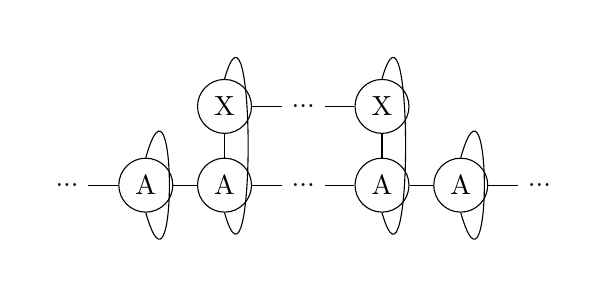
\begin{tikzpicture} [   ]
        	\clip (-1.5,-1) rectangle (5.5,2);
        
        	\node[] (N0) at (-1,0) {...};
        	\node[circle, draw] (N1) at (0,0) {A};
        	\node[circle, draw] (N2) at (1,0) {A};
        	\node[circle, draw] (X2) at (1,1) {X};
        
        	\node[] (N3) at (2 ,0) {...};
        	\node[] (X3) at (2,1) {...};
        
        	\node[circle, draw] (N4) at (3 ,0) {A};
        	\node[circle, draw] (X4) at (3,1) {X};
        
        	\node[circle, draw] (N5) at (4 ,0) {A};
        	\node[] (N6) at (5 ,0) {...};
        
        	\draw  (N0) -- (N1) ;
        
        	\draw  (N1) -- (N2) ;
        	\draw  (N2) -- (N3) ;
        	\draw  (N3) -- (N4) ;
        	\draw  (N4) -- (N5) ;
        	\draw  (N5) -- (N6) ;
        
        
        	\draw  (X2) -- (X3) ;
        	\draw  (X3) -- (X4) ;
        
        	\draw  (N2) -- (X2) ;
        	\draw  (N4) -- (X4) ;
        
        	\draw (X2.north)   .. controls +(0.4,1.4) and +(0.4,-1.4) .. (N2.south);
        	\draw (X4.north)   .. controls +(0.4,1.4) and +(0.4,-1.4) .. (N4.south);
        
        
        	\draw (N1.north)   .. controls +(0.4,1.4) and +(0.4,-1.4) .. (N1.south);
        	\draw (N5.north)   ..  controls +(0.4,1.4) and +(0.4,-1.4)  .. (N5.south);
        \end{tikzpicture}
    }{
        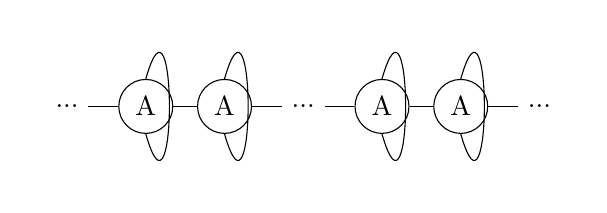
\begin{tikzpicture} [   ]

        	\clip  (-1.5,-3) rectangle (5.5,-1);
        
        
        	\node[] (O0) at (-1,-2) {...};
        	\node[circle, draw] (O1) at (0,-2) {A};
        	\node[circle, draw] (O2) at (1,-2) {A};
        
        
        	\node[] (O3) at (2 ,-2) {...};
        	\node[circle, draw] (O4) at (3 ,-2) {A};
        
        	\node[circle, draw] (O5) at (4 ,-2) {A};
        	\node[] (O6) at (5 ,-2) {...};
        
        	\draw  (O0) -- (O1) ;
        
        	\draw  (O1) -- (O2) ;
        	\draw  (O2) -- (O3) ;
        	\draw  (O3) -- (O4) ;
        	\draw  (O4) -- (O5) ;
        	\draw  (O5) -- (O6) ;
        
        
        	\draw (O2.north)   .. controls +(0.4,1.4) and +(0.4,-1.4) .. (O2.south);
        	\draw (O4.north)   .. controls +(0.4,1.4) and +(0.4,-1.4) .. (O4.south);
        
        
        	\draw (O1.north)   .. controls +(0.4,1.4) and +(0.4,-1.4) .. (O1.south);
        	\draw (O5.north)   ..  controls +(0.4,1.4) and +(0.4,-1.4)  .. (O5.south);
        \end{tikzpicture}
    }
    \label{sm:expecatation_X}
\end{equation}


In the thermodynamic limit there are an infinity number of A to the left and the right. This can be simulated by taking the left and right fixed points of the traced MPO A corresponding to the largest eigenvector $\lambda$.

\begin{equation}
	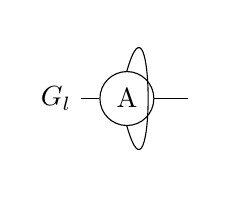
\begin{tikzpicture}[baseline={0cm-0.5*height("$=$")} , scale=0.9] 
	    \clip (-1.4,-1) rectangle (1,1);
        \node[] (N0) at (-1,0) {$G_l$};
        \node[] (N2) at (1,0) {};
    	\node[circle, draw] (N1) at (0,0) {A};
    	\draw  (N0) -- (N1) ;
    	\draw  (N1) -- (N2) ;
    	\draw (N1.north)   .. controls +(0.4,1.4) and +(0.4,-1.4) .. (N1.south);
	\end{tikzpicture}
		= \lambda
	\begin{tikzpicture}[baseline={0cm-0.5*height("$=$")}, scale=0.9 ] 
		\clip (-.4,0.5) rectangle (1,-0.5);
        \node[] (N2) at (1,0) {};
    	\node[] (N1) at (0,0) {$G_l$};
    	\draw  (N1) -- (N2) ;
	\end{tikzpicture}
\end{equation}

\begin{equation}
    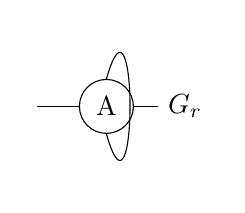
\begin{tikzpicture}[baseline={0cm-0.5*height("$=$")} ] 
        \clip (-1,-1) rectangle (1.4,1);
        \node[] (N0) at (-1,0) {};
        \node[] (N2) at (1,0) {$G_r$};
    	\node[circle, draw] (N1) at (0,0) {A};
    	\draw  (N0) -- (N1) ;
    	\draw  (N1) -- (N2) ;
    	\draw (N1.north)   .. controls +(0.4,1.4) and +(0.4,-1.4) .. (N1.south);
	\end{tikzpicture}
		= \lambda
	\begin{tikzpicture}[baseline={0cm-0.5*height("$=$")} ] 
	    \clip (0,-0.5) rectangle (1.4,0.5);
        \node[] (N2) at (1,0) {$G_l$};
    	\node[] (N1) at (0,0) {};
    	\draw  (N1) -- (N2) ;
	\end{tikzpicture}
\end{equation}

Equation \cref{sm:expecatation_X} can now be easily caclulated:

\begin{equation}
    \Braket{X} = \frac{
        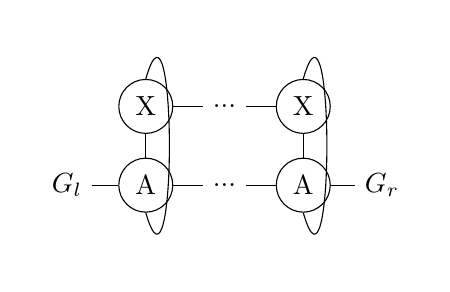
\begin{tikzpicture} [   ]
        	\clip (-0.5,-1) rectangle (4.5,2);
        
        
        	\node[] (N1) at (0,0) {$G_l$};
        	\node[circle, draw] (N2) at (1,0) {A};
        	\node[circle, draw] (X2) at (1,1) {X};
        
        	\node[] (N3) at (2 ,0) {...};
        	\node[] (X3) at (2,1) {...};
        
        	\node[circle, draw] (N4) at (3 ,0) {A};
        	\node[circle, draw] (X4) at (3,1) {X};
        
        	\node[] (N5) at (4 ,0) {$G_r$};

        
        	\draw  (N1) -- (N2) ;
        	\draw  (N2) -- (N3) ;
        	\draw  (N3) -- (N4) ;
        	\draw  (N4) -- (N5) ;

        
   
        	\draw  (X2) -- (X3) ;
        	\draw  (X3) -- (X4) ;
        
        	\draw  (N2) -- (X2) ;
        	\draw  (N4) -- (X4) ;
        
        	\draw (X2.north)   .. controls +(0.4,1.4) and +(0.4,-1.4) .. (N2.south);
        	\draw (X4.north)   .. controls +(0.4,1.4) and +(0.4,-1.4) .. (N4.south);
        
    \end{tikzpicture}
    }{
        \lambda^n 
         \begin{tikzpicture}[baseline={0cm-0.5*height("$=$")} ] 
    	    \clip (-0.5,-0.5) rectangle (1.4,0.5);
            \node[] (N2) at (1,0) {$G_r$};
        	\node[] (N1) at (0,0) {$G_r$};
        	\draw  (N1) -- (N2) ;
    	\end{tikzpicture}
    }
    \label{sm:expecatation_X_2}
\end{equation}